% Lecture Template for ME3001-001-Tristan Hill - Spring 2017 - Fall 2017 - Fall 2020
% Mechanical Engineering Analysis with MATLAB
% Module 2 - Non-Linear Equations
% Topic 3 - The Secant Method

% Document settings

%\documentclass{beamer}                  % for presentation ?
\documentclass[handout]{beamer}  % for handout ?
\usepackage{/home/thill/Documents/lectures/analysis_lectures/analysis_lectures}

\newcommand{\MNUM}{2\hspace{2mm}} % Module number
\newcommand{\TNUM}{3\hspace{2mm}} % Topic number 
\newcommand{\moduletitle}{Nonlinear Equations} % Titles and Stuff
\newcommand{\topictitle}{The Secant Method} 

\newcommand{\sectiontitleI}{Analytical vs. Numerical} % More Titles and Stuff
\newcommand{\sectiontitleII}{Automating Newton-Raphson}
\newcommand{\sectiontitleIII}{Modified Newton-Raphson}
\newcommand{\sectiontitleIV}{The Finite Difference}
\newcommand{\sectiontitleV}{Algorithm Comparison}

\newcommand{\btVFill}{\vskip0pt plus 1filll}

% custom box
\newsavebox{\mybox}

\author{ME3001 - Mechanical Engineering Analysis} 
\title{Lecture Module - \moduletitle}
\date{Mechanical Engineering\vspc Tennessee Technological University}

\begin{document}
	
	\lstset{language=MATLAB,basicstyle=\ttfamily\small,showstringspaces=false}
	
	\frame{\titlepage \center\begin{framed}\Large \textbf{Topic \TNUM - \topictitle}\end{framed} \vspace{5mm}}
	
	% Section 0: Outline
	\frame{
		\large \textbf{Topic \TNUM - \topictitle} \vspace{3mm}\\
		
		\begin{itemize}
			
			\item \sectiontitleI    \vspc % Section I
			\item \sectiontitleII 	\vspc % Section II
			\item \sectiontitleIII 	\vspc %Section III
			\item \sectiontitleIV 	\vspc %Section IV
			
		\end{itemize}
		
	}


\section{\sectiontitleI}

\frame{
	\frametitle{\sectiontitleI}
	
	\textbf{Analytical}
	\begin{itemize}
		\item solution to a problem that can be written in {\bf closed form} 
		\item solution in terms of known functions, constants, etc.  
		\item gives an {\bf exact answer}  \vspcc
	\end{itemize}
	
	\textbf{Numerical}
	\begin{itemize}
		\item an {\bf approximation} to the solution of a mathematical equation
		\item iterative procedure or algorithm
		\item 
	\end{itemize}
	
}

\section{\sectiontitleII}

\frame{
	\frametitle{\sectiontitleII}
	
Our goal is to write a computer program to automate the Newton-Raphson method. We want our program to be (1) robust to different inputs and (2) user friendly. 
	
}


\frame{
  \frametitle{\sectiontitleII}
  
	
	\textbf{The Newton-Raphson method is not \PR{purely numerical}\BK, why?} \\
		\begin{itemize}
			\item  The Equation\vspace{3mm}	\\
			\item  The Derivation\vspace{3mm}	\\
		\end{itemize}
	\textbf{How can we avoid this issue?} \vspace{10mm}\\

	\textbf{{\it Hint:} Think about the title \PR{secant} \BK ...} \vspace{10mm}\\
	
} 

\section{\sectiontitleIII}

\frame{
	\frametitle{\sectiontitleIII}
	
	\textbf{The {\PR secant} method is a modified version of the Newton-Raphson method.} \\
	\begin{multicols}{2}
	Newton-Raphson
	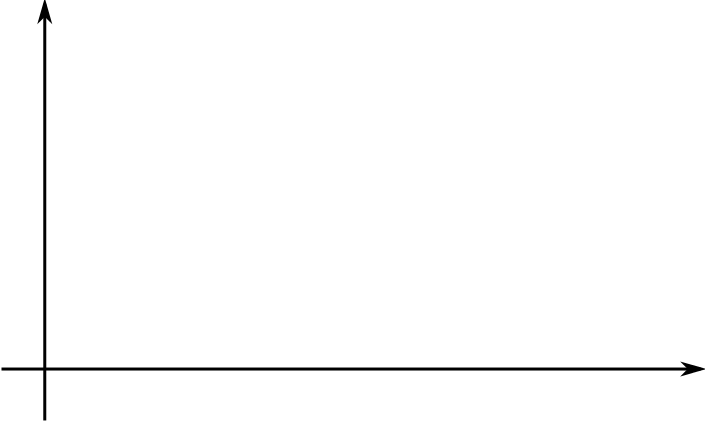
\includegraphics[scale=.22]{lecture4_fig1.png} 
	Secant
	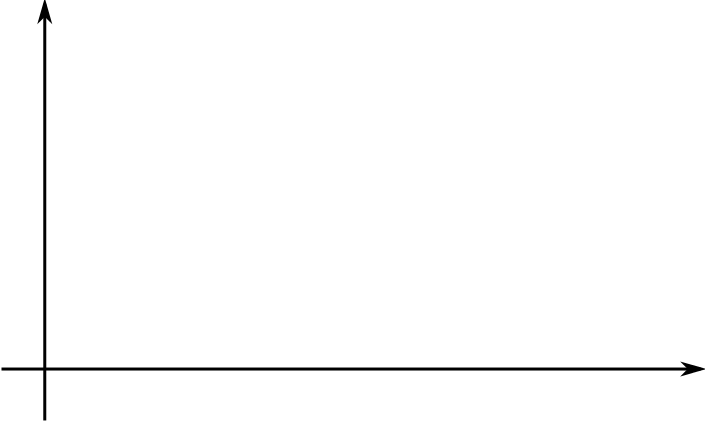
\includegraphics[scale=.22]{lecture4_fig1.png}
	\end{multicols}
	
} 


\frame{
  \frametitle{\sectiontitleIII}
  
	\textbf{The {\PR secant} method is a modified version of the Newton-Raphson method.} \vspace{10mm}\\
\textbf{What are the benefits?} \\
		\begin{itemize}
			\item  \vspace{3mm}
			\item  \vspace{3mm}	
		\end{itemize}
	
\textbf{Are there tradeoffs?} \\
\begin{itemize}
	\item  \vspace{3mm}
	\item  \vspace{3mm}	
\end{itemize}

} 




\section{\sectiontitleIV}

\frame{
	\frametitle{\sectiontitleIV}
	
	This idea or technique is the foundation of a family of methods known as the {\it \PN Finite Difference Methods}.

	\begin{multicols}{3}

	Forward\\
	Difference\\
	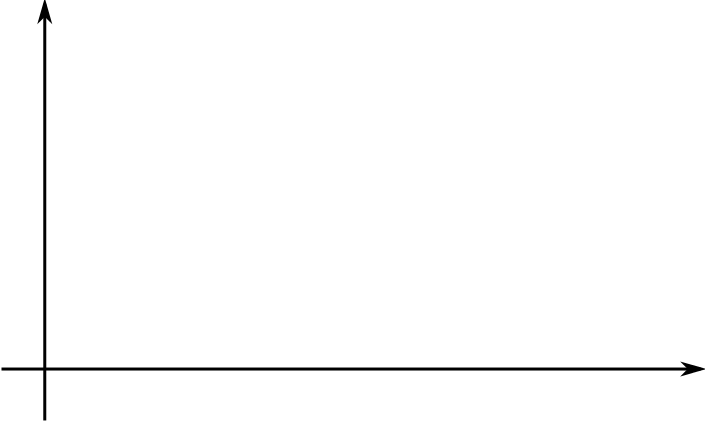
\includegraphics[scale=.14]{lecture4_fig1.png}\\

	Backwards\\
	Difference\\
	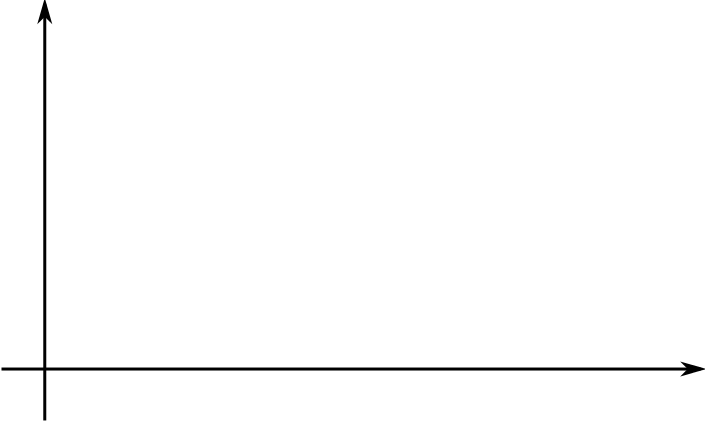
\includegraphics[scale=.14]{lecture4_fig1.png}\\

	Central\\
	Difference\\
	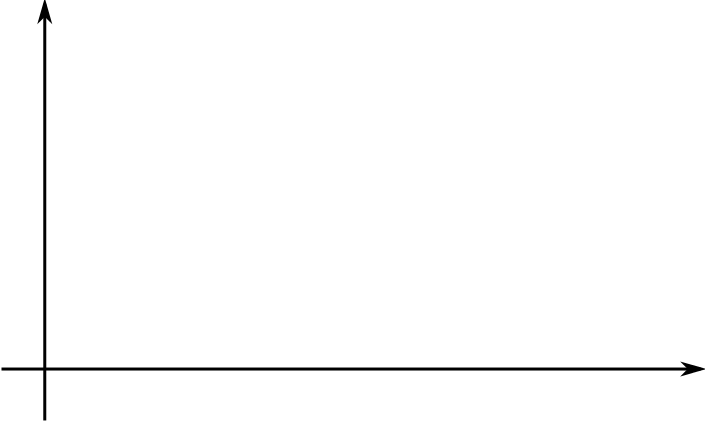
\includegraphics[scale=.14]{lecture4_fig1.png}\\
	
\end{multicols}
}


\end{document}
%\begin{itemize}
%\Large
%	\item \textbf{What does \PR{secant} \K mean?} \vspace{30mm}\\
%	\item \textbf{The Newton-Raphson method is not \PR{purely numerical}\K, why?} \\\\
%		\begin{itemize}
%			\item  The Equation\vspace{30mm}	\\
%			\item  The Derivation\vspace{30mm}	\\
%		\end{itemize}
%	\item \textbf{\LARGE  How can we avoid this issue?}\\\\
%
%\newpage
%	\item \textbf{ \LARGE Introduce the {\it Secant Method (modified Newton-Raphson)}}
%\begin{itemize}	
%	\item \LARGE{Forward Difference}\\\\
%	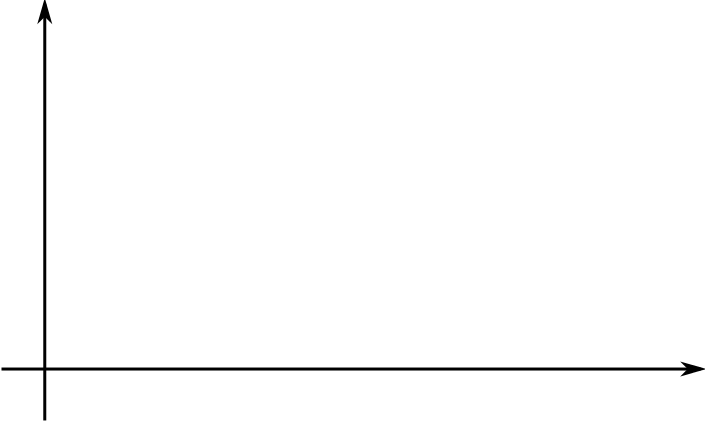
\includegraphics[scale=.35]{lecture4_fig1.png}\\
%	\item \LARGE{Backwards Difference}\\\\
%	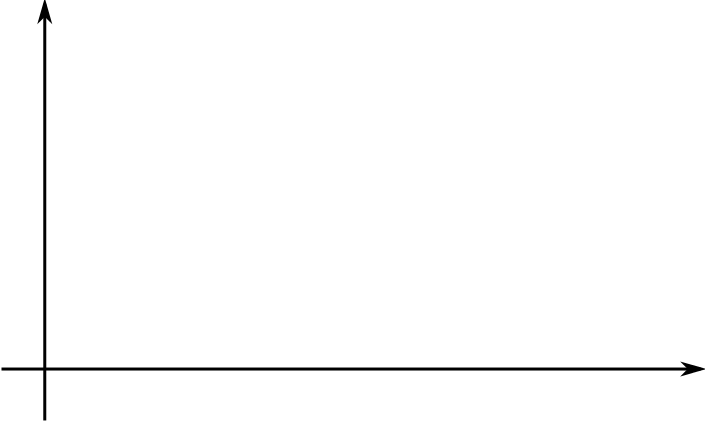
\includegraphics[scale=.35]{lecture4_fig1.png}\\
%	\item \LARGE{Central Difference}\\\\
%	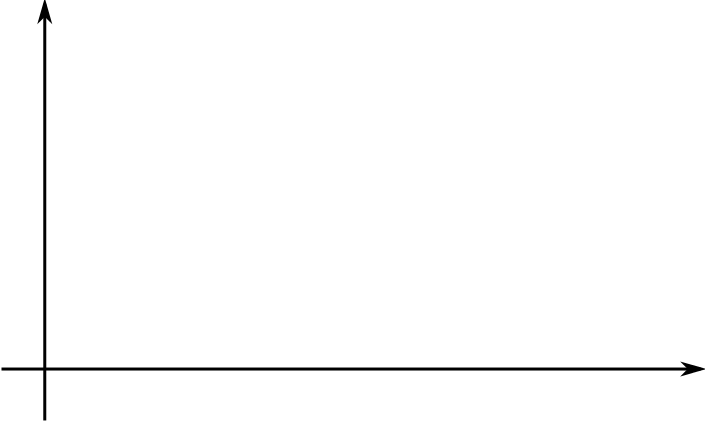
\includegraphics[scale=.35]{lecture4_fig1.png}
%\newpage
%	\item \LARGE{These are know as {\it Finite Difference Approximations} .}\\
%	\item \LARGE{When they are used in the {\it Newton-Raphson} equation this becomes the {\it Secant Method} .}\vspace{25mm}\\
%	
%	\item \LARGE{So what is different about using this method? }\\
%		
%\end{itemize}
%
%		\newpage
%
%\end{itemize}
%\newpage 
%
%% part 2 of the lecture
%\textbf{ \LARGE A Brief Introduction to Optimization } \\
%
%\begin{itemize}
%\Large
%	\item \textbf{\LARGE What is Optimization ?}
%		\begin{itemize}
%			\item Find Local Minima and Maxima \vspace{80mm}	
%			\item Constraints	
%		\end{itemize}
%		\newpage
%		
%	\item \textbf{\LARGE Root finding and Optimization?}
%		\begin{itemize}
%			\item Using the derivative, 4$^{th}$ form of the problem... \vspace{80mm}	
%	
%		\end{itemize}
%	\item \textbf{\LARGE What kind of problems do we solve? Think about the cone we designed a few days ago.}	\\
%			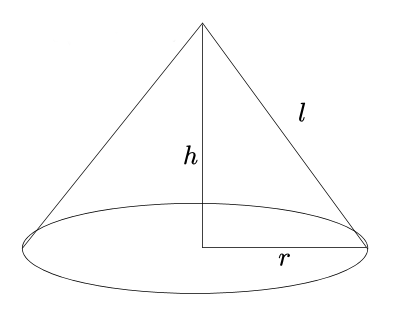
\includegraphics[scale=.5]{lecture4_fig3.png}\hspace{5mm}
%		 \scalebox{1.2}{surface area, $s=\pi r l = \pi r \sqrt{h^2+r^2}$} \\\\
%		  \hspace*{60mm} \scalebox{1.2}{volume, $v=\pi r^2 \frac{h}{3}$} \\\\
%		
%		\newpage
%
%	\item \textbf{\LARGE Optimization Techniques}\\\\
%		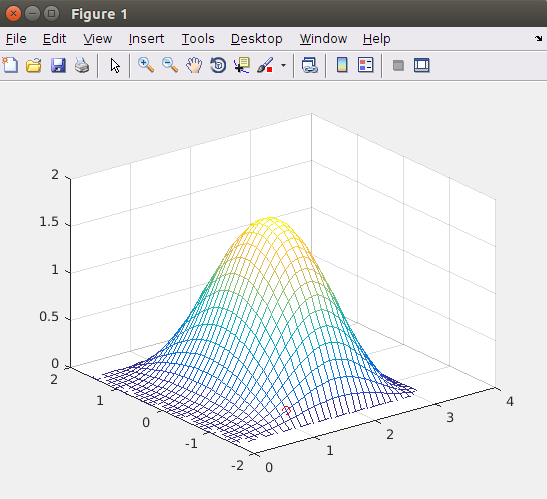
\includegraphics[scale=1]{lecture4_fig2.png}
%		\begin{itemize}
%			\item Brute Force \vspace{30mm}
%			\item Steepest Accent	
%		\end{itemize}
%		\newpage
%
%\end{itemize}
%\textbf{ \LARGE REMINDERS } \\
%
%\begin{itemize}
%
%	\item \textbf{ \LARGE Homework was due Friday but there is a late policy.} \\
%	
%	\item \textbf{ \LARGE The late policy has changed slightly. Please see the syllabus} \\
%	 
%	\item \textbf{ \LARGE MATLAB script from today's lecture will be posted on ilearn. } \\
%		
% \end{itemize}
%
%
%
%
%	
%
%\end{document}
%
%
%
%
%
